% Options for packages loaded elsewhere
\PassOptionsToPackage{unicode}{hyperref}
\PassOptionsToPackage{hyphens}{url}
\documentclass[
]{article}
\usepackage{xcolor}
\usepackage[margin=1in]{geometry}
\usepackage{amsmath,amssymb}
\setcounter{secnumdepth}{-\maxdimen} % remove section numbering
\usepackage{iftex}
\ifPDFTeX
  \usepackage[T1]{fontenc}
  \usepackage[utf8]{inputenc}
  \usepackage{textcomp} % provide euro and other symbols
\else % if luatex or xetex
  \usepackage{unicode-math} % this also loads fontspec
  \defaultfontfeatures{Scale=MatchLowercase}
  \defaultfontfeatures[\rmfamily]{Ligatures=TeX,Scale=1}
\fi
\usepackage{lmodern}
\ifPDFTeX\else
  % xetex/luatex font selection
\fi
% Use upquote if available, for straight quotes in verbatim environments
\IfFileExists{upquote.sty}{\usepackage{upquote}}{}
\IfFileExists{microtype.sty}{% use microtype if available
  \usepackage[]{microtype}
  \UseMicrotypeSet[protrusion]{basicmath} % disable protrusion for tt fonts
}{}
\makeatletter
\@ifundefined{KOMAClassName}{% if non-KOMA class
  \IfFileExists{parskip.sty}{%
    \usepackage{parskip}
  }{% else
    \setlength{\parindent}{0pt}
    \setlength{\parskip}{6pt plus 2pt minus 1pt}}
}{% if KOMA class
  \KOMAoptions{parskip=half}}
\makeatother
\usepackage{longtable,booktabs,array}
\usepackage{calc} % for calculating minipage widths
% Correct order of tables after \paragraph or \subparagraph
\usepackage{etoolbox}
\makeatletter
\patchcmd\longtable{\par}{\if@noskipsec\mbox{}\fi\par}{}{}
\makeatother
% Allow footnotes in longtable head/foot
\IfFileExists{footnotehyper.sty}{\usepackage{footnotehyper}}{\usepackage{footnote}}
\makesavenoteenv{longtable}
\usepackage{graphicx}
\makeatletter
\newsavebox\pandoc@box
\newcommand*\pandocbounded[1]{% scales image to fit in text height/width
  \sbox\pandoc@box{#1}%
  \Gscale@div\@tempa{\textheight}{\dimexpr\ht\pandoc@box+\dp\pandoc@box\relax}%
  \Gscale@div\@tempb{\linewidth}{\wd\pandoc@box}%
  \ifdim\@tempb\p@<\@tempa\p@\let\@tempa\@tempb\fi% select the smaller of both
  \ifdim\@tempa\p@<\p@\scalebox{\@tempa}{\usebox\pandoc@box}%
  \else\usebox{\pandoc@box}%
  \fi%
}
% Set default figure placement to htbp
\def\fps@figure{htbp}
\makeatother
\setlength{\emergencystretch}{3em} % prevent overfull lines
\providecommand{\tightlist}{%
  \setlength{\itemsep}{0pt}\setlength{\parskip}{0pt}}
\usepackage{bookmark}
\IfFileExists{xurl.sty}{\usepackage{xurl}}{} % add URL line breaks if available
\urlstyle{same}
\hypersetup{
  pdftitle={Analysis and visualization},
  hidelinks,
  pdfcreator={LaTeX via pandoc}}

\title{Analysis and visualization}
\author{}
\date{\vspace{-2.5em}2026-01-08}

\begin{document}
\maketitle

This is an R Markdown document for easy access to and recreation of the
figures for the manuscript ``Measuring the health benefits, costs, and
cost-effectiveness of antimicrobial-resistant gonorrhea surveillance in
the United States'', currently in revision at \emph{Lancet Public Health
Americas.}

\section{Figure 1}\label{figure-1}

\begin{figure}
\centering
\pandocbounded{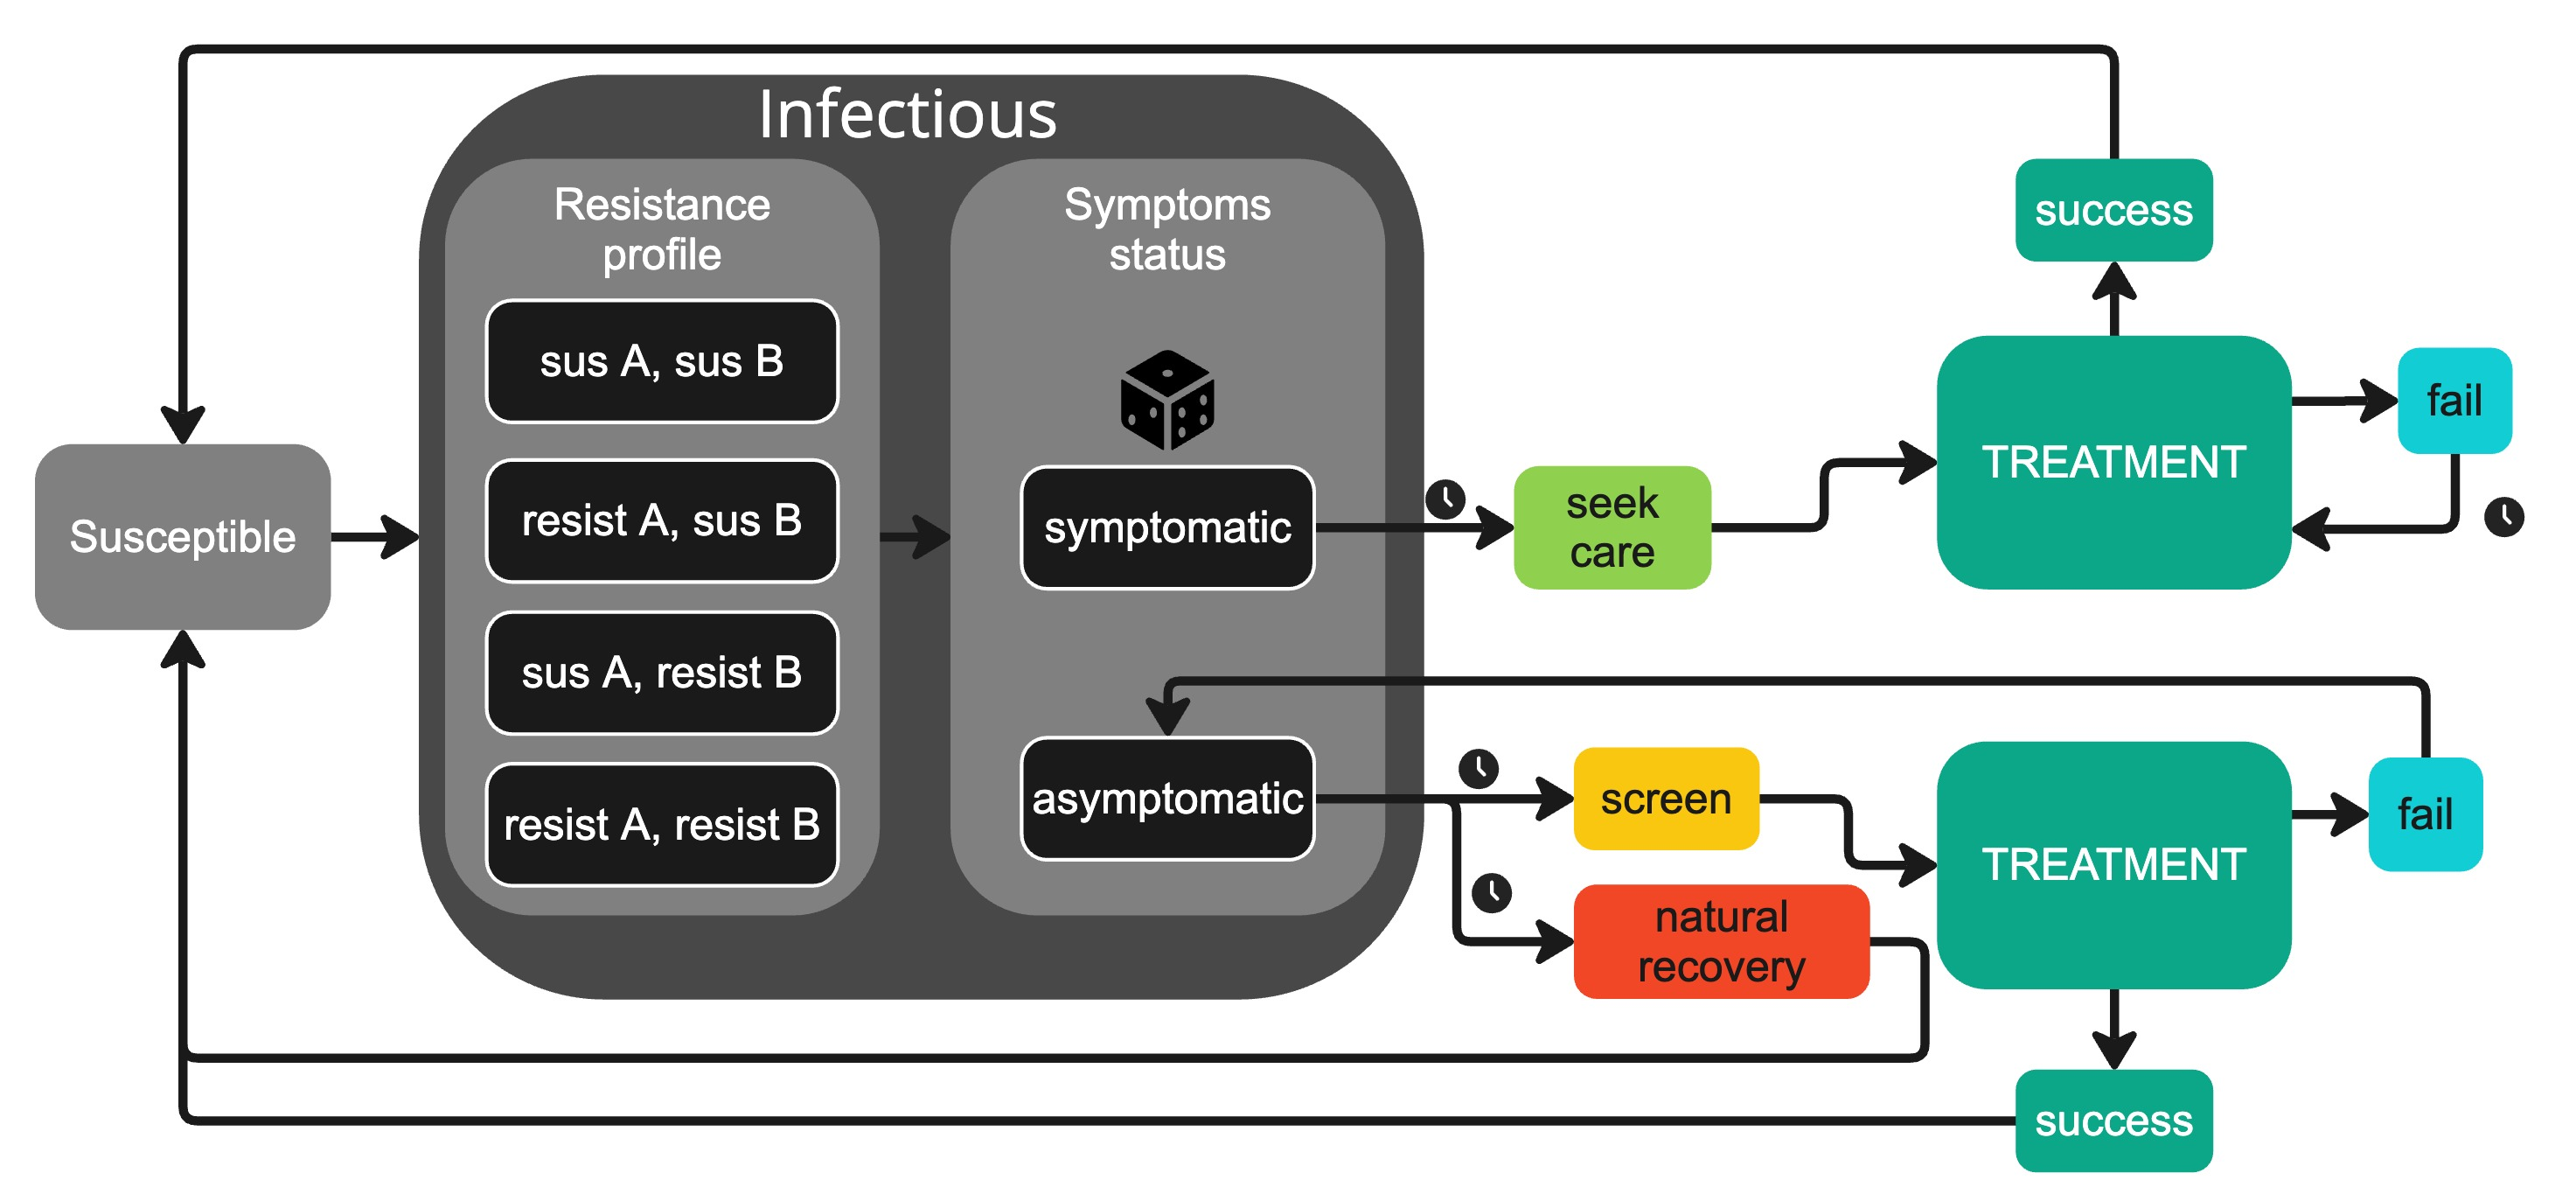
\includegraphics[keepaspectratio]{Figure 1.jpg}}
\caption{\textbf{Figure 1.}}
\end{figure}

\section{Figure 2}\label{figure-2}

\pandocbounded{
\includegraphics[keepaspectratio]{Analysis-and-visualization_files/figure-latex/figure2-1.pdf}}

\begin{longtable}[]{@{}
  >{\raggedright\arraybackslash}p{(\linewidth - 22\tabcolsep) * \real{0.1514}}
  >{\raggedleft\arraybackslash}p{(\linewidth - 22\tabcolsep) * \real{0.0757}}
  >{\raggedleft\arraybackslash}p{(\linewidth - 22\tabcolsep) * \real{0.1036}}
  >{\raggedright\arraybackslash}p{(\linewidth - 22\tabcolsep) * \real{0.0757}}
  >{\raggedright\arraybackslash}p{(\linewidth - 22\tabcolsep) * \real{0.0757}}
  >{\raggedright\arraybackslash}p{(\linewidth - 22\tabcolsep) * \real{0.0876}}
  >{\raggedright\arraybackslash}p{(\linewidth - 22\tabcolsep) * \real{0.0876}}
  >{\raggedleft\arraybackslash}p{(\linewidth - 22\tabcolsep) * \real{0.0598}}
  >{\raggedleft\arraybackslash}p{(\linewidth - 22\tabcolsep) * \real{0.0757}}
  >{\raggedleft\arraybackslash}p{(\linewidth - 22\tabcolsep) * \real{0.0319}}
  >{\raggedleft\arraybackslash}p{(\linewidth - 22\tabcolsep) * \real{0.1155}}
  >{\raggedleft\arraybackslash}p{(\linewidth - 22\tabcolsep) * \real{0.0598}}@{}}
\toprule\noalign{}
\begin{minipage}[b]{\linewidth}\raggedright
\end{minipage} & \begin{minipage}[b]{\linewidth}\raggedleft
Calibration Target
\end{minipage} & \begin{minipage}[b]{\linewidth}\raggedleft
Posterior estimate (mean)
\end{minipage} & \begin{minipage}[b]{\linewidth}\raggedright
Posterior 95\% CI
\end{minipage} & \begin{minipage}[b]{\linewidth}\raggedright
Posterior 50\% CI
\end{minipage} & \begin{minipage}[b]{\linewidth}\raggedright
Target Within 95\% CI?
\end{minipage} & \begin{minipage}[b]{\linewidth}\raggedright
Target Within 50\% CI?
\end{minipage} & \begin{minipage}[b]{\linewidth}\raggedleft
Absolute Error
\end{minipage} & \begin{minipage}[b]{\linewidth}\raggedleft
Relative Error (\%)
\end{minipage} & \begin{minipage}[b]{\linewidth}\raggedleft
Z-score
\end{minipage} & \begin{minipage}[b]{\linewidth}\raggedleft
Posterior Predictive P-value
\end{minipage} & \begin{minipage}[b]{\linewidth}\raggedleft
95\% CI Overlap
\end{minipage} \\
\midrule\noalign{}
\endhead
\bottomrule\noalign{}
\endlastfoot
Prevalence & 4.50 & 4.48 & (3.94, 5.02) & (4.28, 4.67) & TRUE & TRUE &
0.02 & 0.50 & 0.08 & 0.47 & 0.75 \\
Detected cases & 6508.00 & 6440.42 & (5251.75, 7878.00) & (5883.75,
6936.75) & TRUE & TRUE & 67.58 & 1.04 & 0.10 & 0.44 & 0.98 \\
Proportion detected cases symptomatic & 0.68 & 0.68 & (0.65, 0.71) &
(0.67, 0.69) & TRUE & TRUE & 0.00 & 0.18 & -0.08 & 0.54 & 0.62 \\
\end{longtable}

\section{Figure 3}\label{figure-3}

\pandocbounded{
\includegraphics[keepaspectratio]{Analysis-and-visualization_files/figure-latex/figure3-1.pdf}}
\pandocbounded{
\includegraphics[keepaspectratio]{Analysis-and-visualization_files/figure-latex/figure3-2.pdf}}

\section{Figure 4}\label{figure-4}

\pandocbounded{
\includegraphics[keepaspectratio]{Analysis-and-visualization_files/figure-latex/Figure4-1.pdf}}
\pandocbounded{
\includegraphics[keepaspectratio]{Analysis-and-visualization_files/figure-latex/Figure4-2.pdf}}

\section{Figure 5}\label{figure-5}

\pandocbounded{
\includegraphics[keepaspectratio]{Analysis-and-visualization_files/figure-latex/figure5-1.pdf}}

\begin{longtable}[]{@{}
  >{\raggedright\arraybackslash}p{(\linewidth - 8\tabcolsep) * \real{0.2059}}
  >{\raggedright\arraybackslash}p{(\linewidth - 8\tabcolsep) * \real{0.1863}}
  >{\raggedright\arraybackslash}p{(\linewidth - 8\tabcolsep) * \real{0.2549}}
  >{\raggedright\arraybackslash}p{(\linewidth - 8\tabcolsep) * \real{0.1863}}
  >{\raggedright\arraybackslash}p{(\linewidth - 8\tabcolsep) * \real{0.1667}}@{}}
\toprule\noalign{}
\begin{minipage}[b]{\linewidth}\raggedright
\end{minipage} & \begin{minipage}[b]{\linewidth}\raggedright
GISP
\end{minipage} & \begin{minipage}[b]{\linewidth}\raggedright
Randomized Treatment (RT)
\end{minipage} & \begin{minipage}[b]{\linewidth}\raggedright
Test of Cure (TOC)
\end{minipage} & \begin{minipage}[b]{\linewidth}\raggedright
Combo
\end{minipage} \\
\midrule\noalign{}
\endhead
\bottomrule\noalign{}
\endlastfoot
Incidence Mean & 722095.921 & 744986.708 & 759672.086 & 748081.591 \\
Incidence Quantiles & 415122.18, 1225184 & 435195.78, 1262317 & 443702,
1301533 & 435395, 1234573 \\
resistance Mean & 28756.018 & 99272.8630000001 & 155983.158 &
120252.208 \\
Resistance Quantiles & 151, 143318 & 111.97, 592069 & 156.62, 745978 &
98, 584297 \\
Failure Mean & 0.604406028982691 & 7.68185619844353 & 16.1107209437809 &
10.6754909902712 \\
Failure Quantiles & 0.02, 2.13 & 0.01, 44.99 & 0.03, 51.47 & 0.02,
44.15 \\
Ertapenem Mean & 2817.918 & 1390.057 & 668.415 & 508.224 \\
Ertapenem Quantiles & 0, 42129.17 & 0, 12890 & 0, 8805 & 0, 8991.25 \\
\end{longtable}

\begin{verbatim}
## [1] 18.28059
\end{verbatim}

\begin{verbatim}
##     2.5%    97.5% 
## 14.24854 28.46493
\end{verbatim}

\begin{verbatim}
## [1] 18.68125
\end{verbatim}

\begin{verbatim}
##     2.5%    97.5% 
## 14.06936 29.35861
\end{verbatim}

\begin{verbatim}
## [1] 24.30013
\end{verbatim}

\begin{verbatim}
##     2.5%    97.5% 
## 17.29253 40.14487
\end{verbatim}

\begin{verbatim}
## [1] 20.87264
\end{verbatim}

\begin{verbatim}
##     2.5%    97.5% 
## 15.56149 33.83249
\end{verbatim}

\begin{verbatim}
## [1] NA
\end{verbatim}

\begin{verbatim}
##     2.5%    97.5% 
## 147.9210 389.3321
\end{verbatim}

\begin{verbatim}
## [1] 230.6751
\end{verbatim}

\begin{verbatim}
##     2.5%    97.5% 
## 147.1901 400.7693
\end{verbatim}

\begin{verbatim}
## [1] 240.8352
\end{verbatim}

\begin{verbatim}
##     2.5%    97.5% 
## 148.6698 385.5724
\end{verbatim}

\begin{verbatim}
## [1] 229.4356
\end{verbatim}

\begin{verbatim}
##     2.5%    97.5% 
## 145.0009 367.7745
\end{verbatim}

\section{Supplement}\label{supplement}

Validation: results of the partial-rank correlation coefficient (PRCC)
analysis

\begin{longtable}[]{@{}
  >{\raggedright\arraybackslash}p{(\linewidth - 14\tabcolsep) * \real{0.0309}}
  >{\raggedright\arraybackslash}p{(\linewidth - 14\tabcolsep) * \real{0.3196}}
  >{\raggedleft\arraybackslash}p{(\linewidth - 14\tabcolsep) * \real{0.1134}}
  >{\raggedleft\arraybackslash}p{(\linewidth - 14\tabcolsep) * \real{0.1134}}
  >{\raggedleft\arraybackslash}p{(\linewidth - 14\tabcolsep) * \real{0.1134}}
  >{\raggedleft\arraybackslash}p{(\linewidth - 14\tabcolsep) * \real{0.1546}}
  >{\raggedleft\arraybackslash}p{(\linewidth - 14\tabcolsep) * \real{0.0515}}
  >{\raggedleft\arraybackslash}p{(\linewidth - 14\tabcolsep) * \real{0.1031}}@{}}
\caption{Prevalence PRCC}\tabularnewline
\toprule\noalign{}
\begin{minipage}[b]{\linewidth}\raggedright
\end{minipage} & \begin{minipage}[b]{\linewidth}\raggedright
var
\end{minipage} & \begin{minipage}[b]{\linewidth}\raggedleft
est
\end{minipage} & \begin{minipage}[b]{\linewidth}\raggedleft
lower
\end{minipage} & \begin{minipage}[b]{\linewidth}\raggedleft
upper
\end{minipage} & \begin{minipage}[b]{\linewidth}\raggedleft
test.statistic
\end{minipage} & \begin{minipage}[b]{\linewidth}\raggedleft
df
\end{minipage} & \begin{minipage}[b]{\linewidth}\raggedleft
p.value
\end{minipage} \\
\midrule\noalign{}
\endfirsthead
\toprule\noalign{}
\begin{minipage}[b]{\linewidth}\raggedright
\end{minipage} & \begin{minipage}[b]{\linewidth}\raggedright
var
\end{minipage} & \begin{minipage}[b]{\linewidth}\raggedleft
est
\end{minipage} & \begin{minipage}[b]{\linewidth}\raggedleft
lower
\end{minipage} & \begin{minipage}[b]{\linewidth}\raggedleft
upper
\end{minipage} & \begin{minipage}[b]{\linewidth}\raggedleft
test.statistic
\end{minipage} & \begin{minipage}[b]{\linewidth}\raggedleft
df
\end{minipage} & \begin{minipage}[b]{\linewidth}\raggedleft
p.value
\end{minipage} \\
\midrule\noalign{}
\endhead
\bottomrule\noalign{}
\endlastfoot
12 & PercentResistantA & 0.2535614 & 0.1979813 & 0.3091416 & 8.9508162 &
1166 & 0.0000000 \\
11 & activityGroupTransmissionRatio & 0.2033518 & 0.1470944 & 0.2596091
& 7.0919823 & 1166 & 0.0000000 \\
2 & propHighActivity & 0.1808790 & 0.1243689 & 0.2373892 & 6.2800159 &
1166 & 0.0000000 \\
9 & Assortativity & -0.1348897 & -0.1918225 & -0.0779569 & -4.6485276 &
1166 & 0.0000037 \\
4 & NaturalRecoveryTime & 0.1029694 & 0.0458169 & 0.1601219 & 3.5348604
& 1166 & 0.0004240 \\
10 & activityGroupTransferProp & -0.0912771 & -0.1484952 & -0.0340591 &
-3.1298827 & 1166 & 0.0017922 \\
5 & ProbSymptomaticMSM & -0.0843176 & -0.1415709 & -0.0270643 &
-2.8894620 & 1166 & 0.0039304 \\
8 & DelayToRetreatmentMSM & 0.0837688 & 0.0265129 & 0.1410248 &
2.8705219 & 1166 & 0.0041720 \\
3 & TransmissionMSM & 0.0651600 & 0.0078242 & 0.1224958 & 2.2297413 &
1166 & 0.0259545 \\
7 & DelayToSeekCareMSM & 0.0604411 & 0.0030882 & 0.1177940 & 2.0676474 &
1166 & 0.0388934 \\
14 & ImportingBInterval & -0.0601478 & -0.1175017 & -0.0027939 &
-2.0575770 & 1166 & 0.0398527 \\
21 & DrugBTreatmentCost & 0.0556475 & -0.0017214 & 0.1130164 & 1.9031292
& 1166 & 0.0572698 \\
23 & DrugETreatmentCost & -0.0536052 & -0.1109805 & 0.0037701 &
-1.8330794 & 1166 & 0.0670456 \\
19 & StrainTestCost & 0.0520410 & -0.0053390 & 0.1094211 & 1.7794433 &
1166 & 0.0754275 \\
17 & CareCost & 0.0450640 & -0.0123356 & 0.1024635 & 1.5403523 & 1166 &
0.1237458 \\
22 & DrugXTreatmentCost & 0.0384264 & -0.0189891 & 0.0958419 & 1.3131069
& 1166 & 0.1894053 \\
20 & DrugATreatmentCost & 0.0246961 & -0.0327443 & 0.0821365 & 0.8435494
& 1166 & 0.3990942 \\
16 & DSTspecificity & -0.0234547 & -0.0808968 & 0.0339874 & -0.8011231 &
1166 & 0.4232236 \\
13 & BeginImportingB & 0.0226664 & -0.0347768 & 0.0801095 & 0.7741820 &
1166 & 0.4389801 \\
18 & TestCost & -0.0194631 & -0.0769101 & 0.0379840 & -0.6647266 & 1166
& 0.5063568 \\
15 & DSTsensitivity & -0.0185374 & -0.0759855 & 0.0389106 & -0.6331022 &
1166 & 0.5267910 \\
6 & ScreenIntervalMSM & -0.0174241 & -0.0748733 & 0.0400251 & -0.5950655
& 1166 & 0.5519152 \\
1 & InitialInfected & -0.0125112 & -0.0699647 & 0.0449422 & -0.4272516 &
1166 & 0.6692749 \\
\end{longtable}

\begin{longtable}[]{@{}
  >{\raggedright\arraybackslash}p{(\linewidth - 14\tabcolsep) * \real{0.0309}}
  >{\raggedright\arraybackslash}p{(\linewidth - 14\tabcolsep) * \real{0.3196}}
  >{\raggedleft\arraybackslash}p{(\linewidth - 14\tabcolsep) * \real{0.1134}}
  >{\raggedleft\arraybackslash}p{(\linewidth - 14\tabcolsep) * \real{0.1134}}
  >{\raggedleft\arraybackslash}p{(\linewidth - 14\tabcolsep) * \real{0.1134}}
  >{\raggedleft\arraybackslash}p{(\linewidth - 14\tabcolsep) * \real{0.1546}}
  >{\raggedleft\arraybackslash}p{(\linewidth - 14\tabcolsep) * \real{0.0515}}
  >{\raggedleft\arraybackslash}p{(\linewidth - 14\tabcolsep) * \real{0.1031}}@{}}
\caption{Incidence PRCC}\tabularnewline
\toprule\noalign{}
\begin{minipage}[b]{\linewidth}\raggedright
\end{minipage} & \begin{minipage}[b]{\linewidth}\raggedright
var
\end{minipage} & \begin{minipage}[b]{\linewidth}\raggedleft
est
\end{minipage} & \begin{minipage}[b]{\linewidth}\raggedleft
lower
\end{minipage} & \begin{minipage}[b]{\linewidth}\raggedleft
upper
\end{minipage} & \begin{minipage}[b]{\linewidth}\raggedleft
test.statistic
\end{minipage} & \begin{minipage}[b]{\linewidth}\raggedleft
df
\end{minipage} & \begin{minipage}[b]{\linewidth}\raggedleft
p.value
\end{minipage} \\
\midrule\noalign{}
\endfirsthead
\toprule\noalign{}
\begin{minipage}[b]{\linewidth}\raggedright
\end{minipage} & \begin{minipage}[b]{\linewidth}\raggedright
var
\end{minipage} & \begin{minipage}[b]{\linewidth}\raggedleft
est
\end{minipage} & \begin{minipage}[b]{\linewidth}\raggedleft
lower
\end{minipage} & \begin{minipage}[b]{\linewidth}\raggedleft
upper
\end{minipage} & \begin{minipage}[b]{\linewidth}\raggedleft
test.statistic
\end{minipage} & \begin{minipage}[b]{\linewidth}\raggedleft
df
\end{minipage} & \begin{minipage}[b]{\linewidth}\raggedleft
p.value
\end{minipage} \\
\midrule\noalign{}
\endhead
\bottomrule\noalign{}
\endlastfoot
12 & PercentResistantA & 0.2296460 & 0.1737237 & 0.2855683 & 8.0569937 &
1166 & 0.0000000 \\
11 & activityGroupTransmissionRatio & 0.2154684 & 0.1593601 & 0.2715767
& 7.5345234 & 1166 & 0.0000000 \\
10 & activityGroupTransferProp & -0.2018606 & -0.2581357 & -0.1455855 &
-7.0377588 & 1166 & 0.0000000 \\
3 & TransmissionMSM & 0.1835534 & 0.1270718 & 0.2400351 & 6.3760834 &
1166 & 0.0000000 \\
6 & ScreenIntervalMSM & -0.1817040 & -0.2382054 & -0.1252025 &
-6.3096326 & 1166 & 0.0000000 \\
5 & ProbSymptomaticMSM & -0.1523458 & -0.2091330 & -0.0955586 &
-5.2635537 & 1166 & 0.0000002 \\
9 & Assortativity & 0.1377399 & 0.0808296 & 0.1946501 & 4.7486290 & 1166
& 0.0000023 \\
2 & propHighActivity & 0.1184966 & 0.0614435 & 0.1755496 & 4.0749817 &
1166 & 0.0000491 \\
8 & DelayToRetreatmentMSM & 0.0807836 & 0.0235135 & 0.1380538 &
2.7675433 & 1166 & 0.0057374 \\
4 & NaturalRecoveryTime & -0.0793179 & -0.1365948 & -0.0220410 &
-2.7170091 & 1166 & 0.0066850 \\
14 & ImportingBInterval & -0.0713769 & -0.1286882 & -0.0140655 &
-2.4435196 & 1166 & 0.0146923 \\
7 & DelayToSeekCareMSM & 0.0663483 & 0.0090170 & 0.1236796 & 2.2705809 &
1166 & 0.0233541 \\
23 & DrugETreatmentCost & -0.0576198 & -0.1149823 & -0.0002574 &
-1.9708038 & 1166 & 0.0489826 \\
19 & StrainTestCost & 0.0522913 & -0.0050881 & 0.1096706 & 1.7880221 &
1166 & 0.0740320 \\
1 & InitialInfected & -0.0516667 & -0.1090479 & 0.0057145 & -1.7666098 &
1166 & 0.0775552 \\
17 & CareCost & 0.0369661 & -0.0204526 & 0.0943847 & 1.2631336 & 1166 &
0.2067937 \\
21 & DrugBTreatmentCost & 0.0304292 & -0.0270021 & 0.0878605 & 1.0395398
& 1166 & 0.2987693 \\
15 & DSTsensitivity & -0.0246001 & -0.0820406 & 0.0328405 & -0.8402667 &
1166 & 0.4009311 \\
22 & DrugXTreatmentCost & -0.0145497 & -0.0720016 & 0.0429021 &
-0.4968783 & 1166 & 0.6193685 \\
16 & DSTspecificity & -0.0137254 & -0.0711779 & 0.0437271 & -0.4687233 &
1166 & 0.6393551 \\
18 & TestCost & 0.0105212 & -0.0469336 & 0.0679759 & 0.3592831 & 1166 &
0.7194484 \\
20 & DrugATreatmentCost & 0.0060372 & -0.0514196 & 0.0634941 & 0.2061558
& 1166 & 0.8367052 \\
13 & BeginImportingB & -0.0038647 & -0.0613222 & 0.0535928 & -0.1319686
& 1166 & 0.8950319 \\
\end{longtable}

\begin{longtable}[]{@{}
  >{\raggedright\arraybackslash}p{(\linewidth - 14\tabcolsep) * \real{0.0309}}
  >{\raggedright\arraybackslash}p{(\linewidth - 14\tabcolsep) * \real{0.3196}}
  >{\raggedleft\arraybackslash}p{(\linewidth - 14\tabcolsep) * \real{0.1134}}
  >{\raggedleft\arraybackslash}p{(\linewidth - 14\tabcolsep) * \real{0.1134}}
  >{\raggedleft\arraybackslash}p{(\linewidth - 14\tabcolsep) * \real{0.1134}}
  >{\raggedleft\arraybackslash}p{(\linewidth - 14\tabcolsep) * \real{0.1546}}
  >{\raggedleft\arraybackslash}p{(\linewidth - 14\tabcolsep) * \real{0.0515}}
  >{\raggedleft\arraybackslash}p{(\linewidth - 14\tabcolsep) * \real{0.1031}}@{}}
\caption{Symptomatic Proportion PRCC}\tabularnewline
\toprule\noalign{}
\begin{minipage}[b]{\linewidth}\raggedright
\end{minipage} & \begin{minipage}[b]{\linewidth}\raggedright
var
\end{minipage} & \begin{minipage}[b]{\linewidth}\raggedleft
est
\end{minipage} & \begin{minipage}[b]{\linewidth}\raggedleft
lower
\end{minipage} & \begin{minipage}[b]{\linewidth}\raggedleft
upper
\end{minipage} & \begin{minipage}[b]{\linewidth}\raggedleft
test.statistic
\end{minipage} & \begin{minipage}[b]{\linewidth}\raggedleft
df
\end{minipage} & \begin{minipage}[b]{\linewidth}\raggedleft
p.value
\end{minipage} \\
\midrule\noalign{}
\endfirsthead
\toprule\noalign{}
\begin{minipage}[b]{\linewidth}\raggedright
\end{minipage} & \begin{minipage}[b]{\linewidth}\raggedright
var
\end{minipage} & \begin{minipage}[b]{\linewidth}\raggedleft
est
\end{minipage} & \begin{minipage}[b]{\linewidth}\raggedleft
lower
\end{minipage} & \begin{minipage}[b]{\linewidth}\raggedleft
upper
\end{minipage} & \begin{minipage}[b]{\linewidth}\raggedleft
test.statistic
\end{minipage} & \begin{minipage}[b]{\linewidth}\raggedleft
df
\end{minipage} & \begin{minipage}[b]{\linewidth}\raggedleft
p.value
\end{minipage} \\
\midrule\noalign{}
\endhead
\bottomrule\noalign{}
\endlastfoot
7 & DelayToSeekCareMSM & 0.5846784 & 0.5380648 & 0.6312920 & 24.6095407
& 1166 & 0.0000000 \\
5 & ProbSymptomaticMSM & 0.3045867 & 0.2498589 & 0.3593145 & 10.9194862
& 1166 & 0.0000000 \\
12 & PercentResistantA & 0.2229015 & 0.1668891 & 0.2789138 & 7.8077954 &
1166 & 0.0000000 \\
14 & ImportingBInterval & -0.1544772 & -0.2112454 & -0.0977090 &
-5.3389799 & 1166 & 0.0000001 \\
8 & DelayToRetreatmentMSM & 0.1505846 & 0.0937819 & 0.2073874 &
5.2012842 & 1166 & 0.0000002 \\
11 & activityGroupTransmissionRatio & 0.1314284 & 0.0744689 & 0.1883879
& 4.5271222 & 1166 & 0.0000066 \\
6 & ScreenIntervalMSM & -0.1241793 & -0.1811925 & -0.0671661 &
-4.2733950 & 1166 & 0.0000208 \\
3 & TransmissionMSM & 0.1095215 & 0.0524092 & 0.1666338 & 3.7624349 &
1166 & 0.0001766 \\
9 & Assortativity & 0.1040184 & 0.0468722 & 0.1611646 & 3.5712622 & 1166
& 0.0003697 \\
4 & NaturalRecoveryTime & -0.1020879 & -0.1592456 & -0.0449301 &
-3.5042766 & 1166 & 0.0004752 \\
15 & DSTsensitivity & -0.0946308 & -0.1518309 & -0.0374307 & -3.2458996
& 1166 & 0.0012041 \\
17 & CareCost & 0.0630594 & 0.0057158 & 0.1204029 & 2.1575667 & 1166 &
0.0311653 \\
10 & activityGroupTransferProp & -0.0525981 & -0.1099765 & 0.0047803 &
-1.7985425 & 1166 & 0.0723496 \\
21 & DrugBTreatmentCost & 0.0398068 & -0.0176055 & 0.0972192 & 1.3603520
& 1166 & 0.1739815 \\
13 & BeginImportingB & 0.0372399 & -0.0201782 & 0.0946580 & 1.2725041 &
1166 & 0.2034478 \\
20 & DrugATreatmentCost & -0.0371133 & -0.0945317 & 0.0203050 &
-1.2681731 & 1166 & 0.2049893 \\
1 & InitialInfected & -0.0348305 & -0.0922536 & 0.0225925 & -1.1900716 &
1166 & 0.2342605 \\
22 & DrugXTreatmentCost & -0.0318961 & -0.0893248 & 0.0255326 &
-1.0897025 & 1166 & 0.2760694 \\
19 & StrainTestCost & 0.0247802 & -0.0326601 & 0.0822204 & 0.8464214 &
1166 & 0.3974914 \\
23 & DrugETreatmentCost & -0.0174700 & -0.0749192 & 0.0399791 &
-0.5966362 & 1166 & 0.5508661 \\
2 & propHighActivity & -0.0138701 & -0.0713225 & 0.0435823 & -0.4736653
& 1166 & 0.6358273 \\
16 & DSTspecificity & -0.0132560 & -0.0707089 & 0.0441968 & -0.4526907 &
1166 & 0.6508557 \\
18 & TestCost & -0.0102659 & -0.0677208 & 0.0471890 & -0.3505662 & 1166
& 0.7259772 \\
\end{longtable}

\begin{longtable}[]{@{}
  >{\raggedright\arraybackslash}p{(\linewidth - 14\tabcolsep) * \real{0.0309}}
  >{\raggedright\arraybackslash}p{(\linewidth - 14\tabcolsep) * \real{0.3196}}
  >{\raggedleft\arraybackslash}p{(\linewidth - 14\tabcolsep) * \real{0.1134}}
  >{\raggedleft\arraybackslash}p{(\linewidth - 14\tabcolsep) * \real{0.1134}}
  >{\raggedleft\arraybackslash}p{(\linewidth - 14\tabcolsep) * \real{0.1134}}
  >{\raggedleft\arraybackslash}p{(\linewidth - 14\tabcolsep) * \real{0.1546}}
  >{\raggedleft\arraybackslash}p{(\linewidth - 14\tabcolsep) * \real{0.0515}}
  >{\raggedleft\arraybackslash}p{(\linewidth - 14\tabcolsep) * \real{0.1031}}@{}}
\caption{Costs PRCC}\tabularnewline
\toprule\noalign{}
\begin{minipage}[b]{\linewidth}\raggedright
\end{minipage} & \begin{minipage}[b]{\linewidth}\raggedright
var
\end{minipage} & \begin{minipage}[b]{\linewidth}\raggedleft
est
\end{minipage} & \begin{minipage}[b]{\linewidth}\raggedleft
lower
\end{minipage} & \begin{minipage}[b]{\linewidth}\raggedleft
upper
\end{minipage} & \begin{minipage}[b]{\linewidth}\raggedleft
test.statistic
\end{minipage} & \begin{minipage}[b]{\linewidth}\raggedleft
df
\end{minipage} & \begin{minipage}[b]{\linewidth}\raggedleft
p.value
\end{minipage} \\
\midrule\noalign{}
\endfirsthead
\toprule\noalign{}
\begin{minipage}[b]{\linewidth}\raggedright
\end{minipage} & \begin{minipage}[b]{\linewidth}\raggedright
var
\end{minipage} & \begin{minipage}[b]{\linewidth}\raggedleft
est
\end{minipage} & \begin{minipage}[b]{\linewidth}\raggedleft
lower
\end{minipage} & \begin{minipage}[b]{\linewidth}\raggedleft
upper
\end{minipage} & \begin{minipage}[b]{\linewidth}\raggedleft
test.statistic
\end{minipage} & \begin{minipage}[b]{\linewidth}\raggedleft
df
\end{minipage} & \begin{minipage}[b]{\linewidth}\raggedleft
p.value
\end{minipage} \\
\midrule\noalign{}
\endhead
\bottomrule\noalign{}
\endlastfoot
12 & PercentResistantA & 0.2198044 & 0.1637516 & 0.2758571 & 7.6937614 &
1166 & 0.0000000 \\
11 & activityGroupTransmissionRatio & 0.1753205 & 0.1187525 & 0.2318884
& 6.0808059 & 1166 & 0.0000000 \\
6 & ScreenIntervalMSM & -0.1574026 & -0.2141443 & -0.1006610 &
-5.4426322 & 1166 & 0.0000001 \\
10 & activityGroupTransferProp & -0.1478093 & -0.2046361 & -0.0909825 &
-5.1032614 & 1166 & 0.0000004 \\
17 & CareCost & 0.1238503 & 0.0668347 & 0.1808658 & 4.2618966 & 1166 &
0.0000219 \\
3 & TransmissionMSM & 0.1238213 & 0.0668055 & 0.1808370 & 4.2608827 &
1166 & 0.0000220 \\
2 & propHighActivity & 0.1132104 & 0.0561219 & 0.1702989 & 3.8907806 &
1166 & 0.0001056 \\
14 & ImportingBInterval & -0.0680948 & -0.1254194 & -0.0107703 &
-2.3306264 & 1166 & 0.0199429 \\
5 & ProbSymptomaticMSM & 0.0617498 & 0.0044016 & 0.1190981 & 2.1125871 &
1166 & 0.0348482 \\
19 & StrainTestCost & 0.0521692 & -0.0052105 & 0.1095488 & 1.7838361 &
1166 & 0.0747103 \\
23 & DrugETreatmentCost & -0.0368407 & -0.0942596 & 0.0205782 &
-1.2588454 & 1166 & 0.2083382 \\
15 & DSTsensitivity & -0.0240695 & -0.0815107 & 0.0333718 & -0.8221319 &
1166 & 0.4111699 \\
8 & DelayToRetreatmentMSM & 0.0240356 & -0.0334057 & 0.0814769 &
0.8209742 & 1166 & 0.4118288 \\
9 & Assortativity & 0.0210214 & -0.0364238 & 0.0784666 & 0.7179715 &
1166 & 0.4729187 \\
16 & DSTspecificity & -0.0200762 & -0.0775225 & 0.0373701 & -0.6856749 &
1166 & 0.4930544 \\
21 & DrugBTreatmentCost & 0.0193749 & -0.0380722 & 0.0768220 & 0.6617145
& 1166 & 0.5082850 \\
13 & BeginImportingB & 0.0181673 & -0.0392811 & 0.0756157 & 0.6204561 &
1166 & 0.5350788 \\
1 & InitialInfected & -0.0176459 & -0.0750949 & 0.0398031 & -0.6026440 &
1166 & 0.5468627 \\
4 & NaturalRecoveryTime & 0.0154806 & -0.0419704 & 0.0729316 & 0.5286750
& 1166 & 0.5971315 \\
20 & DrugATreatmentCost & 0.0093548 & -0.0481006 & 0.0668102 & 0.3194515
& 1166 & 0.7494414 \\
22 & DrugXTreatmentCost & 0.0063750 & -0.0510817 & 0.0638318 & 0.2176901
& 1166 & 0.8277087 \\
7 & DelayToSeekCareMSM & 0.0052532 & -0.0522040 & 0.0627103 & 0.1793808
& 1166 & 0.8576699 \\
18 & TestCost & 0.0045369 & -0.0529204 & 0.0619942 & 0.1549226 & 1166 &
0.8769092 \\
\end{longtable}

\begin{longtable}[]{@{}
  >{\raggedright\arraybackslash}p{(\linewidth - 14\tabcolsep) * \real{0.0309}}
  >{\raggedright\arraybackslash}p{(\linewidth - 14\tabcolsep) * \real{0.3196}}
  >{\raggedleft\arraybackslash}p{(\linewidth - 14\tabcolsep) * \real{0.1134}}
  >{\raggedleft\arraybackslash}p{(\linewidth - 14\tabcolsep) * \real{0.1134}}
  >{\raggedleft\arraybackslash}p{(\linewidth - 14\tabcolsep) * \real{0.1134}}
  >{\raggedleft\arraybackslash}p{(\linewidth - 14\tabcolsep) * \real{0.1546}}
  >{\raggedleft\arraybackslash}p{(\linewidth - 14\tabcolsep) * \real{0.0515}}
  >{\raggedleft\arraybackslash}p{(\linewidth - 14\tabcolsep) * \real{0.1031}}@{}}
\caption{QALYs PRCC}\tabularnewline
\toprule\noalign{}
\begin{minipage}[b]{\linewidth}\raggedright
\end{minipage} & \begin{minipage}[b]{\linewidth}\raggedright
var
\end{minipage} & \begin{minipage}[b]{\linewidth}\raggedleft
est
\end{minipage} & \begin{minipage}[b]{\linewidth}\raggedleft
lower
\end{minipage} & \begin{minipage}[b]{\linewidth}\raggedleft
upper
\end{minipage} & \begin{minipage}[b]{\linewidth}\raggedleft
test.statistic
\end{minipage} & \begin{minipage}[b]{\linewidth}\raggedleft
df
\end{minipage} & \begin{minipage}[b]{\linewidth}\raggedleft
p.value
\end{minipage} \\
\midrule\noalign{}
\endfirsthead
\toprule\noalign{}
\begin{minipage}[b]{\linewidth}\raggedright
\end{minipage} & \begin{minipage}[b]{\linewidth}\raggedright
var
\end{minipage} & \begin{minipage}[b]{\linewidth}\raggedleft
est
\end{minipage} & \begin{minipage}[b]{\linewidth}\raggedleft
lower
\end{minipage} & \begin{minipage}[b]{\linewidth}\raggedleft
upper
\end{minipage} & \begin{minipage}[b]{\linewidth}\raggedleft
test.statistic
\end{minipage} & \begin{minipage}[b]{\linewidth}\raggedleft
df
\end{minipage} & \begin{minipage}[b]{\linewidth}\raggedleft
p.value
\end{minipage} \\
\midrule\noalign{}
\endhead
\bottomrule\noalign{}
\endlastfoot
7 & DelayToSeekCareMSM & 0.5190788 & 0.4699680 & 0.5681896 & 20.7374556
& 1166 & 0.0000000 \\
12 & PercentResistantA & 0.2542642 & 0.1986946 & 0.3098337 & 8.9773342 &
1166 & 0.0000000 \\
11 & activityGroupTransmissionRatio & 0.1947824 & 0.1384250 & 0.2511398
& 6.7810654 & 1166 & 0.0000000 \\
5 & ProbSymptomaticMSM & 0.1823259 & 0.1258311 & 0.2388207 & 6.3319715 &
1166 & 0.0000000 \\
10 & activityGroupTransferProp & -0.1667266 & -0.2233803 & -0.1100730 &
-5.7739893 & 1166 & 0.0000000 \\
3 & TransmissionMSM & 0.1530299 & 0.0962487 & 0.2098110 & 5.2877524 &
1166 & 0.0000001 \\
2 & propHighActivity & 0.1303775 & 0.0734100 & 0.1873450 & 4.4902948 &
1166 & 0.0000078 \\
6 & ScreenIntervalMSM & -0.1104149 & -0.1675215 & -0.0533083 &
-3.7935033 & 1166 & 0.0001562 \\
14 & ImportingBInterval & -0.1003102 & -0.1574783 & -0.0431421 &
-3.4426318 & 1166 & 0.0005965 \\
8 & DelayToRetreatmentMSM & 0.0953444 & 0.0381482 & 0.1525406 &
3.2706005 & 1166 & 0.0011046 \\
19 & StrainTestCost & 0.0660775 & 0.0087452 & 0.1234098 & 2.2612731 &
1166 & 0.0239260 \\
23 & DrugETreatmentCost & -0.0637800 & -0.1211209 & -0.0064391 &
-2.1823222 & 1166 & 0.0292848 \\
15 & DSTsensitivity & -0.0586369 & -0.1159960 & -0.0012779 & -2.0057115
& 1166 & 0.0451177 \\
17 & CareCost & 0.0570996 & -0.0002646 & 0.1144638 & 1.9529510 & 1166 &
0.0510644 \\
9 & Assortativity & 0.0459118 & -0.0114856 & 0.1033091 & 1.5693921 &
1166 & 0.1168279 \\
21 & DrugBTreatmentCost & 0.0406167 & -0.0167938 & 0.0980272 & 1.3880720
& 1166 & 0.1653803 \\
18 & TestCost & -0.0326525 & -0.0900797 & 0.0247748 & -1.1155704 & 1166
& 0.2648359 \\
16 & DSTspecificity & -0.0315958 & -0.0890250 & 0.0258334 & -1.0794332 &
1166 & 0.2806179 \\
20 & DrugATreatmentCost & -0.0278146 & -0.0852502 & 0.0296211 &
-0.9501439 & 1166 & 0.3422360 \\
1 & InitialInfected & -0.0186771 & -0.0761250 & 0.0387708 & -0.6378728 &
1166 & 0.5236817 \\
13 & BeginImportingB & 0.0169695 & -0.0404802 & 0.0744191 & 0.5795359 &
1166 & 0.5623396 \\
4 & NaturalRecoveryTime & -0.0110275 & -0.0684819 & 0.0464269 &
-0.3765762 & 1166 & 0.7065571 \\
22 & DrugXTreatmentCost & 0.0090731 & -0.0483825 & 0.0665286 & 0.3098285
& 1166 & 0.7567468 \\
\end{longtable}

\pandocbounded{\includegraphics[keepaspectratio]{Analysis-and-visualization_files/figure-latex/fitnessCostSA-1.pdf}}
\pandocbounded{\includegraphics[keepaspectratio]{Analysis-and-visualization_files/figure-latex/fitnessCostSA-2.pdf}}
\pandocbounded{\includegraphics[keepaspectratio]{Analysis-and-visualization_files/figure-latex/fitnessCostSA-3.pdf}}
\pandocbounded{\includegraphics[keepaspectratio]{Analysis-and-visualization_files/figure-latex/fitnessCostSA-4.pdf}}
\pandocbounded{\includegraphics[keepaspectratio]{Analysis-and-visualization_files/figure-latex/fitnessCostSA-5.pdf}}
\pandocbounded{\includegraphics[keepaspectratio]{Analysis-and-visualization_files/figure-latex/fitnessCostSA-6.pdf}}
\pandocbounded{\includegraphics[keepaspectratio]{Analysis-and-visualization_files/figure-latex/fitnessCostSA-7.pdf}}
\pandocbounded{\includegraphics[keepaspectratio]{Analysis-and-visualization_files/figure-latex/fitnessCostSA-8.pdf}}
\pandocbounded{\includegraphics[keepaspectratio]{Analysis-and-visualization_files/figure-latex/fitnessCostSA-9.pdf}}
\pandocbounded{\includegraphics[keepaspectratio]{Analysis-and-visualization_files/figure-latex/fitnessCostSA-10.pdf}}
\pandocbounded{\includegraphics[keepaspectratio]{Analysis-and-visualization_files/figure-latex/fitnessCostSA-11.pdf}}
\pandocbounded{\includegraphics[keepaspectratio]{Analysis-and-visualization_files/figure-latex/fitnessCostSA-12.pdf}}

\end{document}
